%%%%%%%%%%%%%%%%%%%%%%%%%%%%%%%%%%%%%%%%%%%%%%%%%%%%%%%%%%%%%%%%%%%%%%%%%%%%%%%%%%%%%%%%%%%%%%%%%%%%%%%%%%%%%%%%%%%%%%%%%%%%%%%%%%%%%%%%%%%%%%%%%%%%%%%%%%%%%%%%%%%
% Written By Michael Brodskiy
% Class: Honors Inquiry — Twentieth Century Espionage (HONR1310)
% Professor: J. Burds
%%%%%%%%%%%%%%%%%%%%%%%%%%%%%%%%%%%%%%%%%%%%%%%%%%%%%%%%%%%%%%%%%%%%%%%%%%%%%%%%%%%%%%%%%%%%%%%%%%%%%%%%%%%%%%%%%%%%%%%%%%%%%%%%%%%%%%%%%%%%%%%%%%%%%%%%%%%%%%%%%%%

\documentclass[12pt]{article} 
\usepackage{alphalph}
\usepackage[utf8]{inputenc}
\usepackage[russian,english]{babel}
\usepackage{titling}
\usepackage{amsmath}
\usepackage{graphicx}
\usepackage{enumitem}
\usepackage{amssymb}
\usepackage[super]{nth}
\usepackage{everysel}
\usepackage{ragged2e}
\usepackage{geometry}
\usepackage{multicol}
\usepackage{fancyhdr}
\usepackage{cancel}
\usepackage{siunitx}
\geometry{top=1.0in,bottom=1.0in,left=1.0in,right=1.0in}
\newcommand{\subtitle}[1]{%
  \posttitle{%
    \par\end{center}
    \begin{center}\large#1\end{center}
    \vskip0.5em}%

}
\usepackage{hyperref}
\hypersetup{
colorlinks=true,
linkcolor=blue,
filecolor=magenta,      
urlcolor=blue,
citecolor=blue,
}


\title{The Great Game}
\date{\today}
\author{Michael Brodskiy\\ \small Professor: J. Burds}

\begin{document}

\maketitle

\begin{itemize}

  \item Conflict between England and Russia for supremacy in Central Asia (1813—1907)

  \item Russia did not have a goal equivalent to ``manifest destiny'', instead they wanted to maintain security

    \begin{itemize}

      \item Stephen Wade claims: ``The core of the Russian expansionist plan was to gradually invade and absorb nations contiguous to its heartland''

    \end{itemize}

  \item Wilhelm Stieber — Chief of Intelligence under Bismarck in Germany

    \begin{itemize}

      \item ``\ldots the first national intelligence chief [in Germany] to use agents to monitor and control the press, the banks, business, and industry''

    \end{itemize}

  \item British fears involved the sepoys: In 1836, there were only 17,000 British troops in India, and of these 1,400 were invalids — ``Common sense dictated that a revolt would be hard to contain''

  \item British views of Russian advances into Central Asia:

    \begin{itemize}

      \item ``That great, grim, shadowy power, which sits brooding over Europe and Asia, and of which no man knows really whether it be strong or weak, whether its people be a young race yet to play a great part in the world's history, or men, as Diderot has described them, as rotten before they are ripe; that dark, silent Russian Czar, the hater of freedom, the foe of every people struggling to cast off oppression. . . . ''

    \end{itemize}

  \item Russian views of British advances into Central Asia:

    \begin{itemize}

      \item ``The position of Russia in Central Asia is that of all civilized states which are brought into contact with half-savage nomadic populations, deficient in any fixed social organization. Under such circumstances, it always happens that the more civilized state is forced, in the interest of the security of its frontier and commercial relations, to exercise a certain ascendancy over those whose turbulent and unsettled character make them undesirable neighbors.''

    \end{itemize}

  \item Bradley Mayhew wrote: “[Secret] Agents posing as scholars, explorers, merchants—even Muslim preachers and Buddhist pilgrims—crisscrossed the mountains, mapping them, spying on each other, courting local rulers, staking claims like dogs in a vacant lot.”

  \item Colin Mazkenzie produced many of the first accurate South Asian maps 

  \item The Russo-Turkish War (1877—1878)

    \begin{figure}[h!]
      \centering 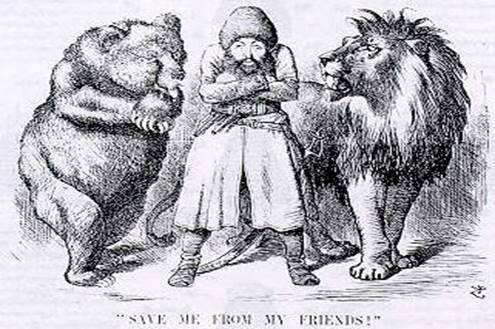
\includegraphics{images/AfghanEmir.jpg}
      \caption{Afghan Emir Sher Ali and his ``friends'' — The British Lion and the Russian Bear}
    \end{figure}

  \item The Russian Conquest of Khiva

    \begin{itemize}

      \item Russian General Skobelev — ``The Butcher of Khiva''

        \begin{itemize}

          \item ``The ablest single commander'' in the world between 1870—1914

          \item ``Russia for Russians''

        \end{itemize}

        \begin{figure}[h!]
          \centering 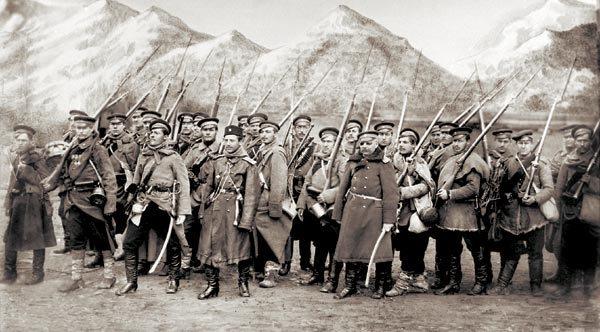
\includegraphics[width=.7\textwidth]{images/SkobelevTroops.png}
          \caption{Skobelev's Troops}
        \end{figure}

      \item The Lomakin Massacre

        \begin{itemize}

          \item In 1879, a force of 4,000 cavalry and infantry under General Lomakin marched across the desert to attack the Teke at Geok-Tepe

        \end{itemize}

      \item The Battle of Geok-Tepe

        \begin{itemize}

          \item General Mikhail Skobelev was sent to Turkestan in December 1880 to avenge the humiliating defeat and to free Russian prisoners

          \item 6,000 Russian soldiers vs 25,000 Turkmen defenders in a heavily fortified town

          \item The siege of Geok Tepe lasted 23 days, after which the city was taken by storm

          \item Russian forces dug a tunnel underneath a portion of the wall, then detonated a mine underneath the main fortress wall.

          \item 24 January 1881, the mine was detonated; Once the fortress was breached, the Russian troops stormed into the city

            \begin{figure}[h!]
              \centering 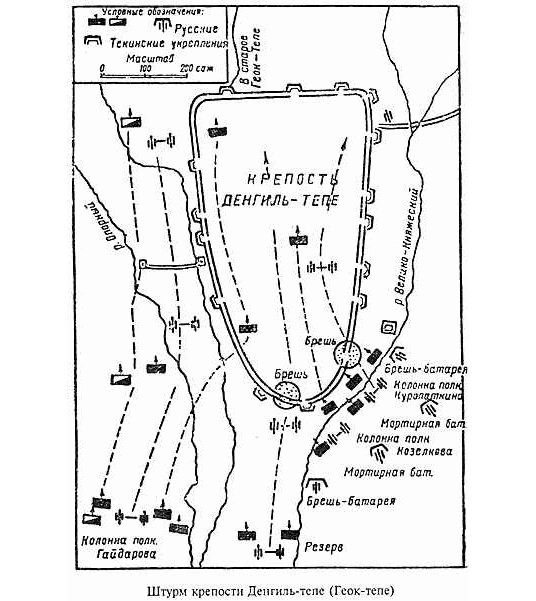
\includegraphics[width=.6\textwidth]{images/GeokTepe.png}
              \caption{The Siege of Geok-Tepe}
            \end{figure}

        \end{itemize}

      \item Vasily Vereshchagin's paintings shed light on the atrocities committed in the war — Skobelev is demoted for this, and sent to Minsk

    \end{itemize}

  \item Thus, the Great Game was a ``dress rehearsal'' for the Cold War

\end{itemize}

\end{document}

